\chapter{針對不同使用情境進行最佳化}
\label{chp:5}



如第四章所述,系統設計上具有靈活度,我們可以透過改變硬體指向、硬體數量、朗博次方,來改變系統的表現。因此,我們可以針對不同的使用情境,給出最佳的系統設計,本章節於依序於\ref{chp:optimize}章定義最佳化問題,並於章中針對\ref{chp:scenario}章中室內定位的例子,於\ref{chp:optimize_case}章給出最佳系統設計。







% --------------------------------------

\section{最佳化流程}
\label{chp:optimize}

最佳化變數的部分,包含朗博次方$Mp,M\ell$、硬體指向$^{P}\boldsymbol{V}_p,^{L}\boldsymbol{V}_l$與硬體數量$P,L$,而其中每個硬體皆有朗博次方與硬體指向需要定義,因此最佳化的變數量又會根據硬體數量而改變,使得最佳化難度高。為了簡化這個變數數量與變數本身相關的問題,我們將硬體數量於於最佳化流程的最開始定義,參考流程圖\ref{pic:optimize_flow},硬體數量確定後,針對朗博次方與指向的最佳化問題則可利用基因演算法(Genetic Algorithm,以下簡稱GA)求解。而透過迭代改變硬體數量,我們可以得到不同硬體數量對應的最佳設計,以及該設計的目標函數。擁有這些資訊,即可透過人類決策者介入選擇最合適的硬體數量,在系統表現以及硬體成本中進行取捨。

\begin{figure}[h!]
    \centering
    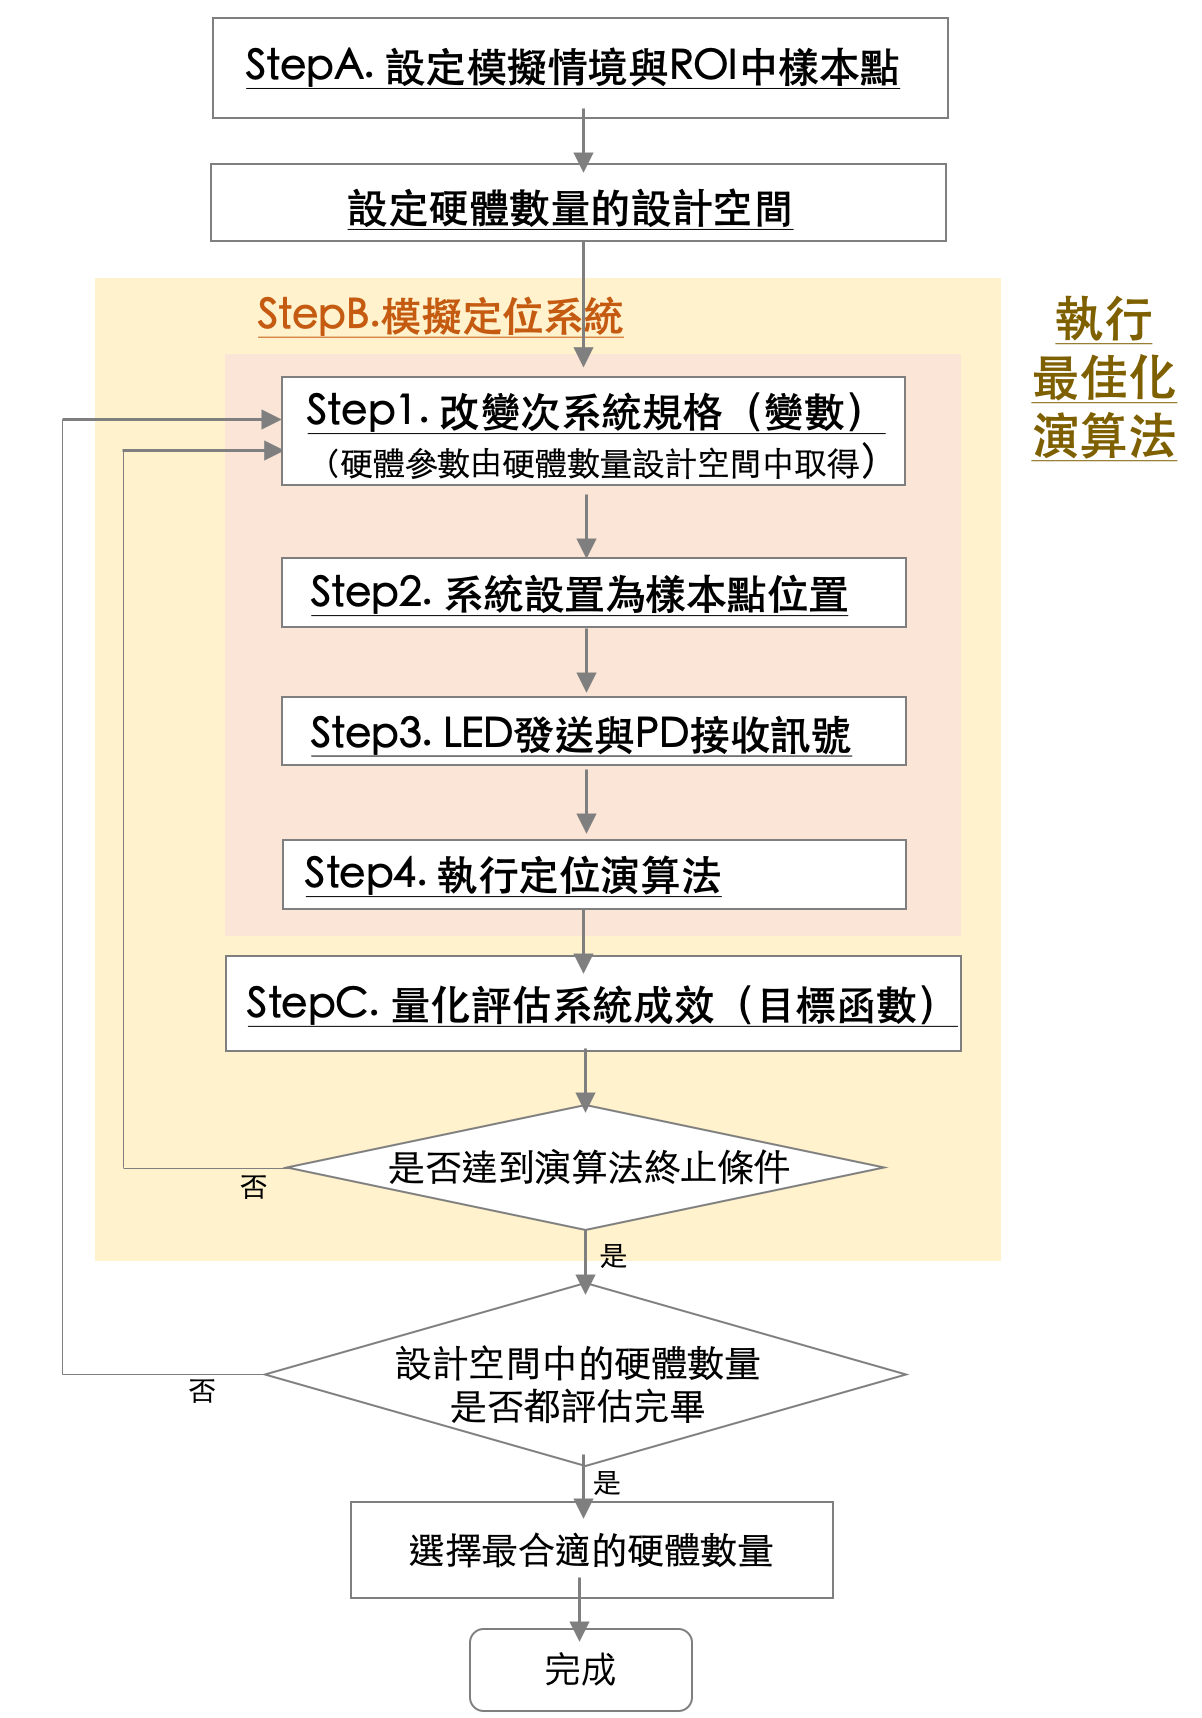
\includegraphics[width=13cm]{ch5pic/optimize_flow.png}
    \caption{最佳化流程圖}
    \label{pic:optimize_flow}
\end{figure}

    \subsection{目標函數}

    我們的最佳化目標,是希望使系統表現更好,而評估方式可以參考\ref{chp:system_perform}章所述,目標是讓在容許範圍內的樣本點比例越高越好。因此,在硬體總數設定為$P,L$的情況下,最佳化目標函數$f$呈現於式\ref{eqn:objective}

    \begin{equation}
        \label{eqn:objective}
        \begin{aligned}
        \underset{^{P}\boldsymbol{V}_p, ^{L}\boldsymbol{V}_l,Ml,Mp}{\operatorname{minimize}} 
        \quad f = 
        \frac{\sum_{i=1}^{K}F(k)}{K}  \\
        \text{Where }F(k)=
        \begin{cases}
            _{k}e<To&,1\\
            else&,0
        \end{cases}
        \end{aligned}
    \end{equation}

    \begin{align*} \text{where }
        &p=1,2,...,P\\&l=1,2,...,L
    \end{align*}


    \subsection{最佳化變數}

    最佳化變數的部分,包含朗博次方$Mp,M\ell$、硬體指向$^{P}\boldsymbol{V}_p,^{L}\boldsymbol{V}_l$與硬體數量$P,L$,而其中每個硬體皆有朗博次方與硬體指向需要定義,因此最佳化的變數量又會根據硬體數量而改變,變數總數為$2+2\times(L+P)$。


    \begin{figure}[h!]
        \centering
        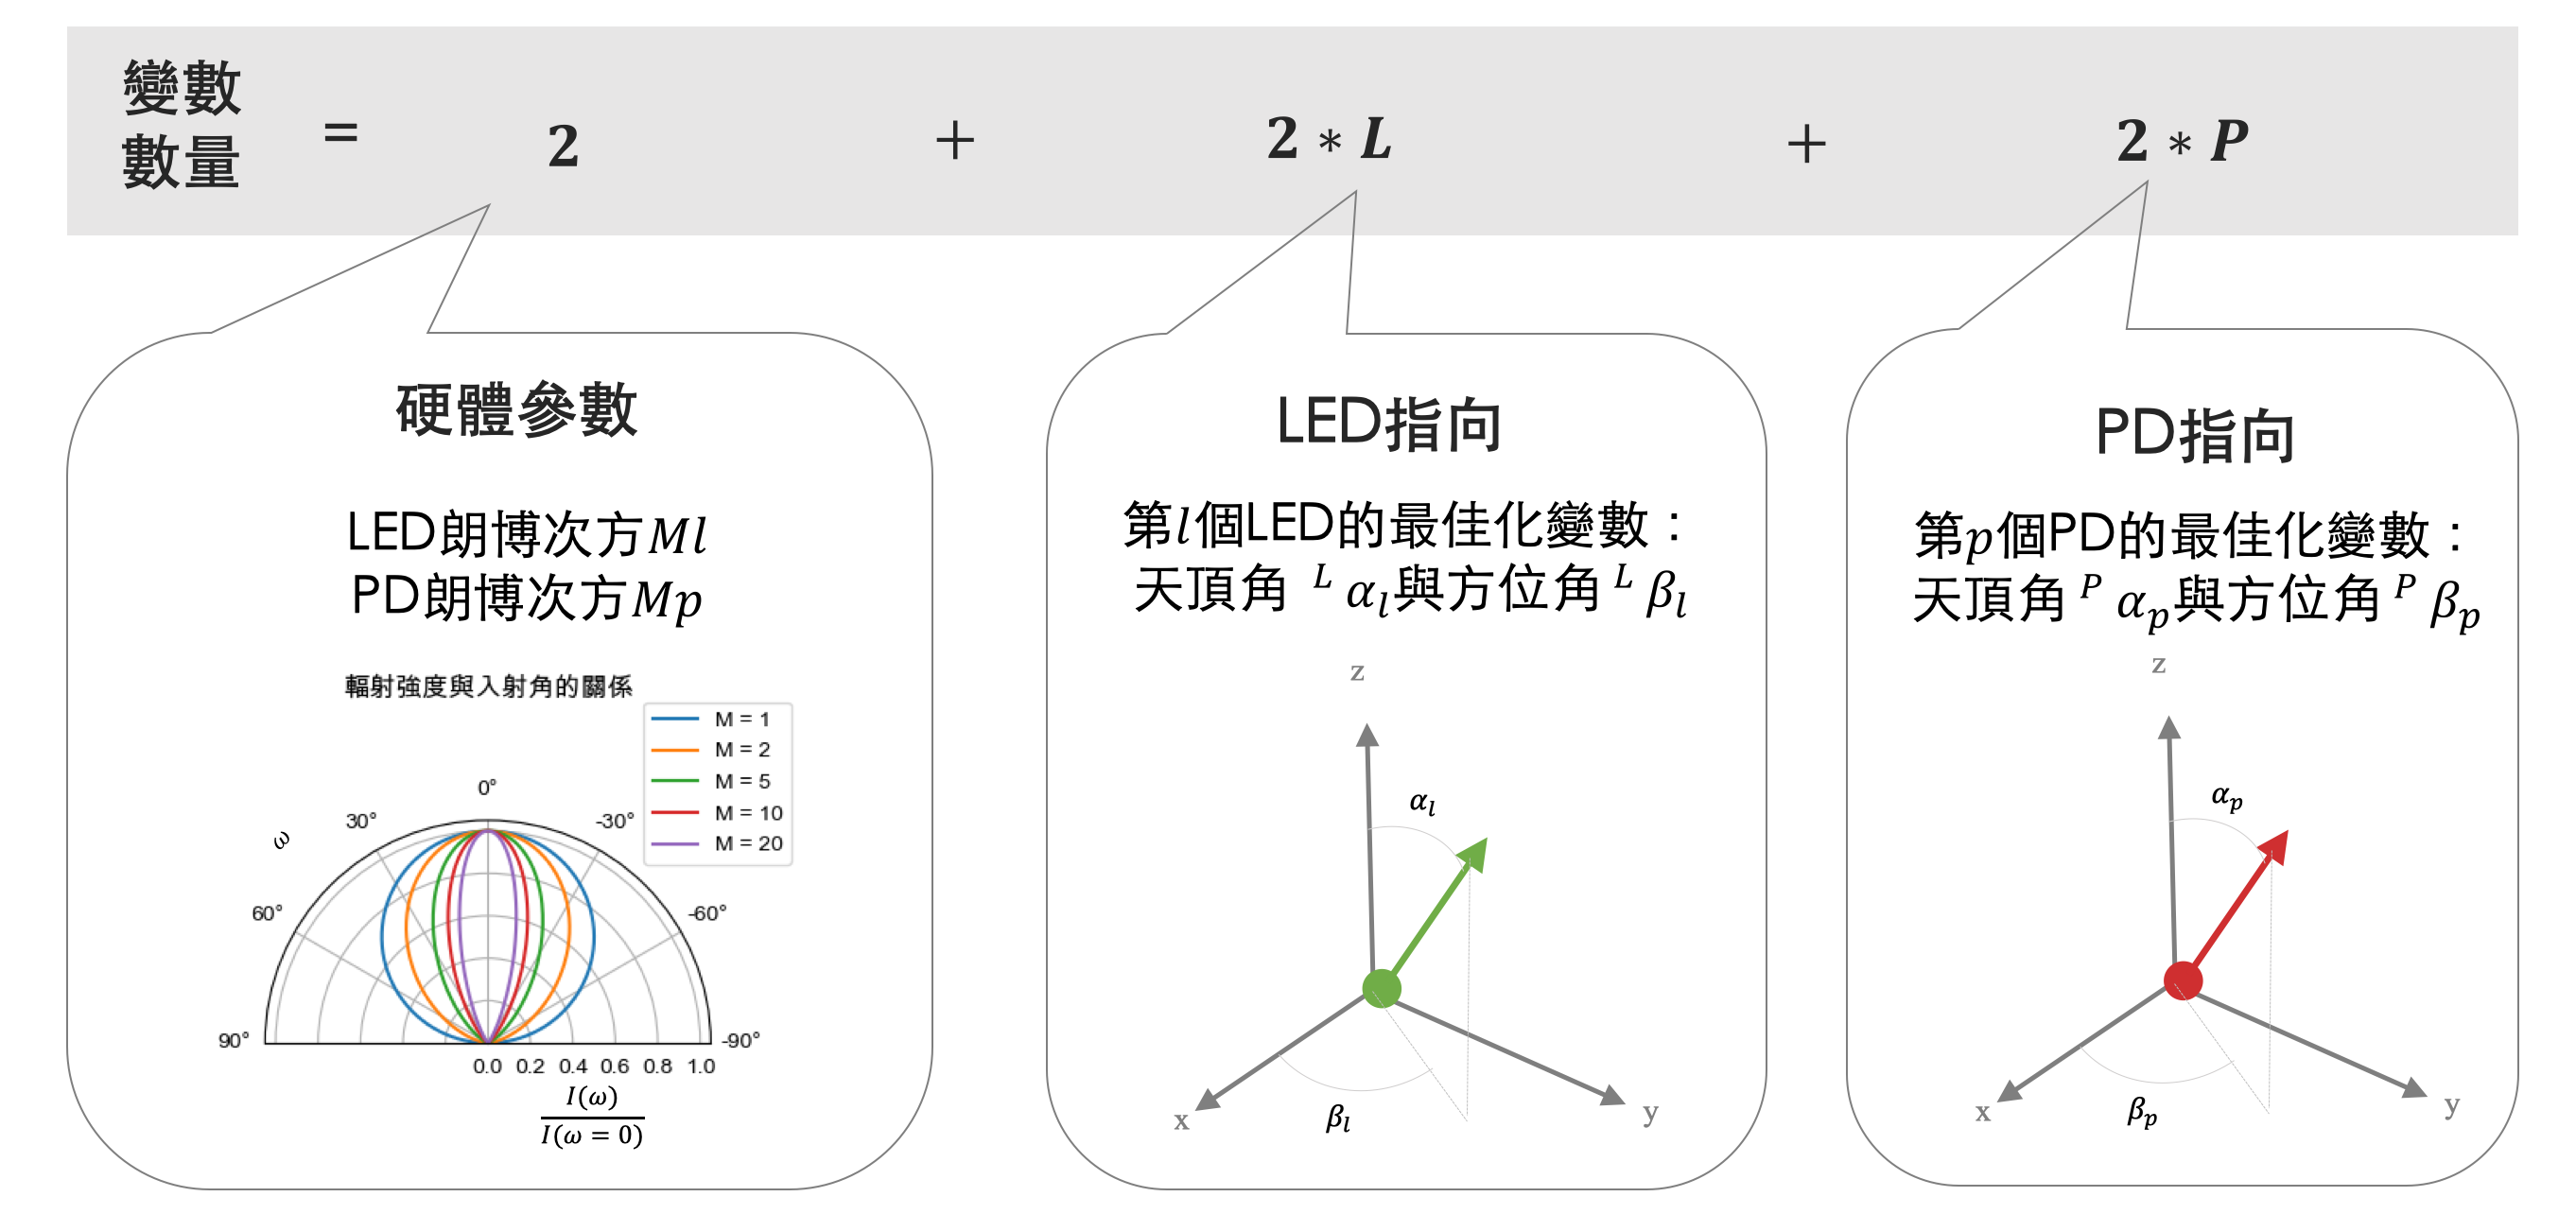
\includegraphics[width=15cm]{ch5pic/optimize_variable.png}
        \caption{最佳化變數}
        \label{pic:optimize_variable}
    \end{figure}



% --------------------------------------
\section{案例}
\label{chp:optimize_case}

    \subsection{室內空間的案例}

    我們最佳化的目標情境參考\ref{chp:scenario}章,為一包含平移樣本與旋轉樣本的的室內空間,而以下圖\ref{pic:opt_result}呈現硬體數量分別為$P=L=5$以及$P=L=10$時,朗博次方與硬體指向的最佳化結果。

    \begin{figure}[h!]
        \centering
        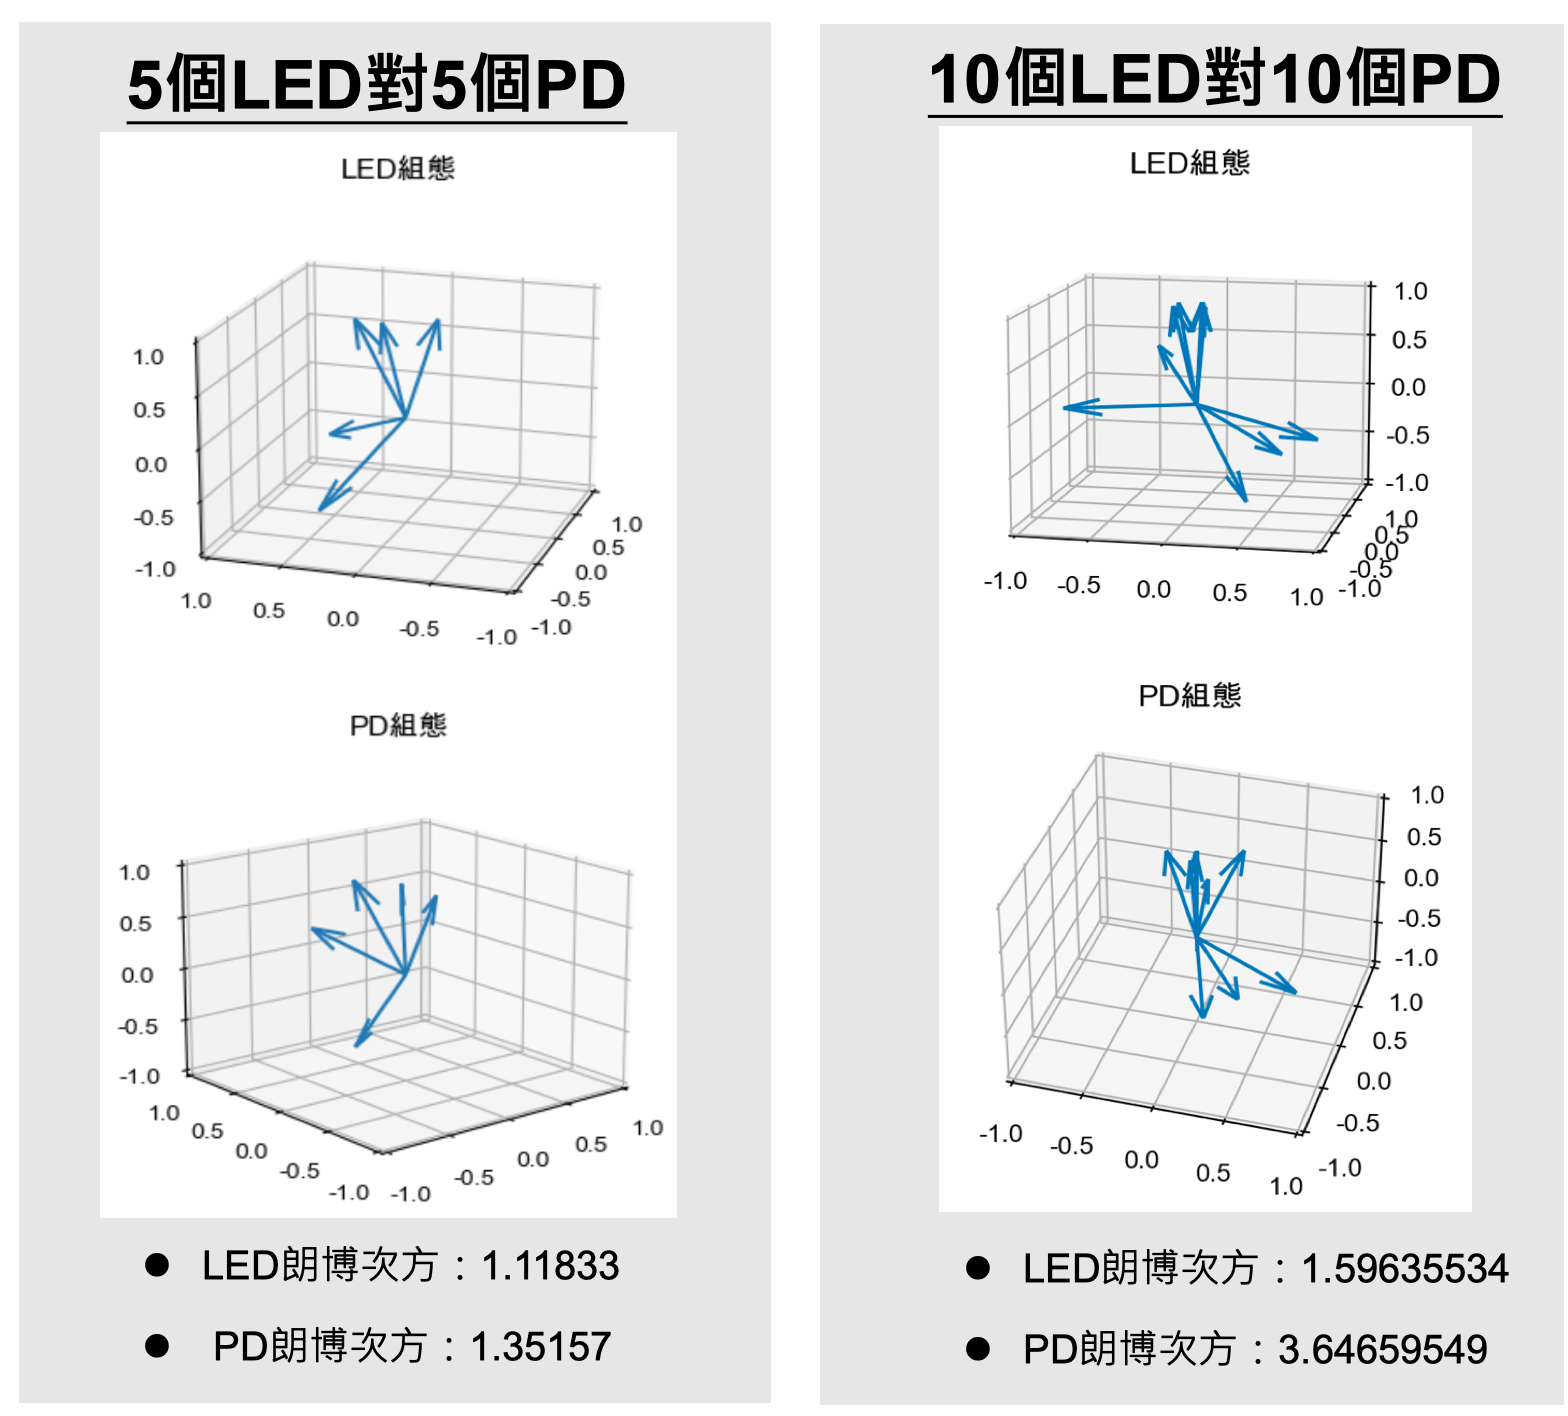
\includegraphics[width=15cm]{ch5pic/opt_result.png}
        \caption{最佳化結果}
        \label{pic:opt_result}
    \end{figure}

    觀察這兩個系統設計的差別,在硬體數量少的時候,為了讓空間中的最多個樣本點可讀到訊號,因此朗博次方較小,捨棄了對出入射角敏感度。

    % \subsection{以目標物為中心的案例}


% --------------------------------------
\section{結論}

本章節提出一流程,針對不同使用情境,進行朗博次方$Mp,M\ell$、硬體指向$^{P}\boldsymbol{V}_p,^{L}\boldsymbol{V}_l$與硬體數量$P,L$的最佳化。透過設定不同的情境、不同的參數,我們可以得到最適合的朗博次方與硬體擺設設計,也知道不同硬體數量的表現。由此資訊,再進行硬體的購買以及硬體系統的搭建,便可以減少硬體系統重複測試的麻煩。







% --------------------------------------


% \subsection{情境設定}

% 需先定義此量測工況中觀察者座標系的ROI(Region of Interest),擁有此資訊後,將此範圍切割成數個樣本點位置(圖\ref{pic:testpoint})。我們將觀察者的PD座標系固定,將目標物的LED座標系放置於各樣本點,所有樣本點的平均誤差即為量測表現,誤差愈小代表量測表現愈好。

% \begin{figure}[ht]
%     \centering
%     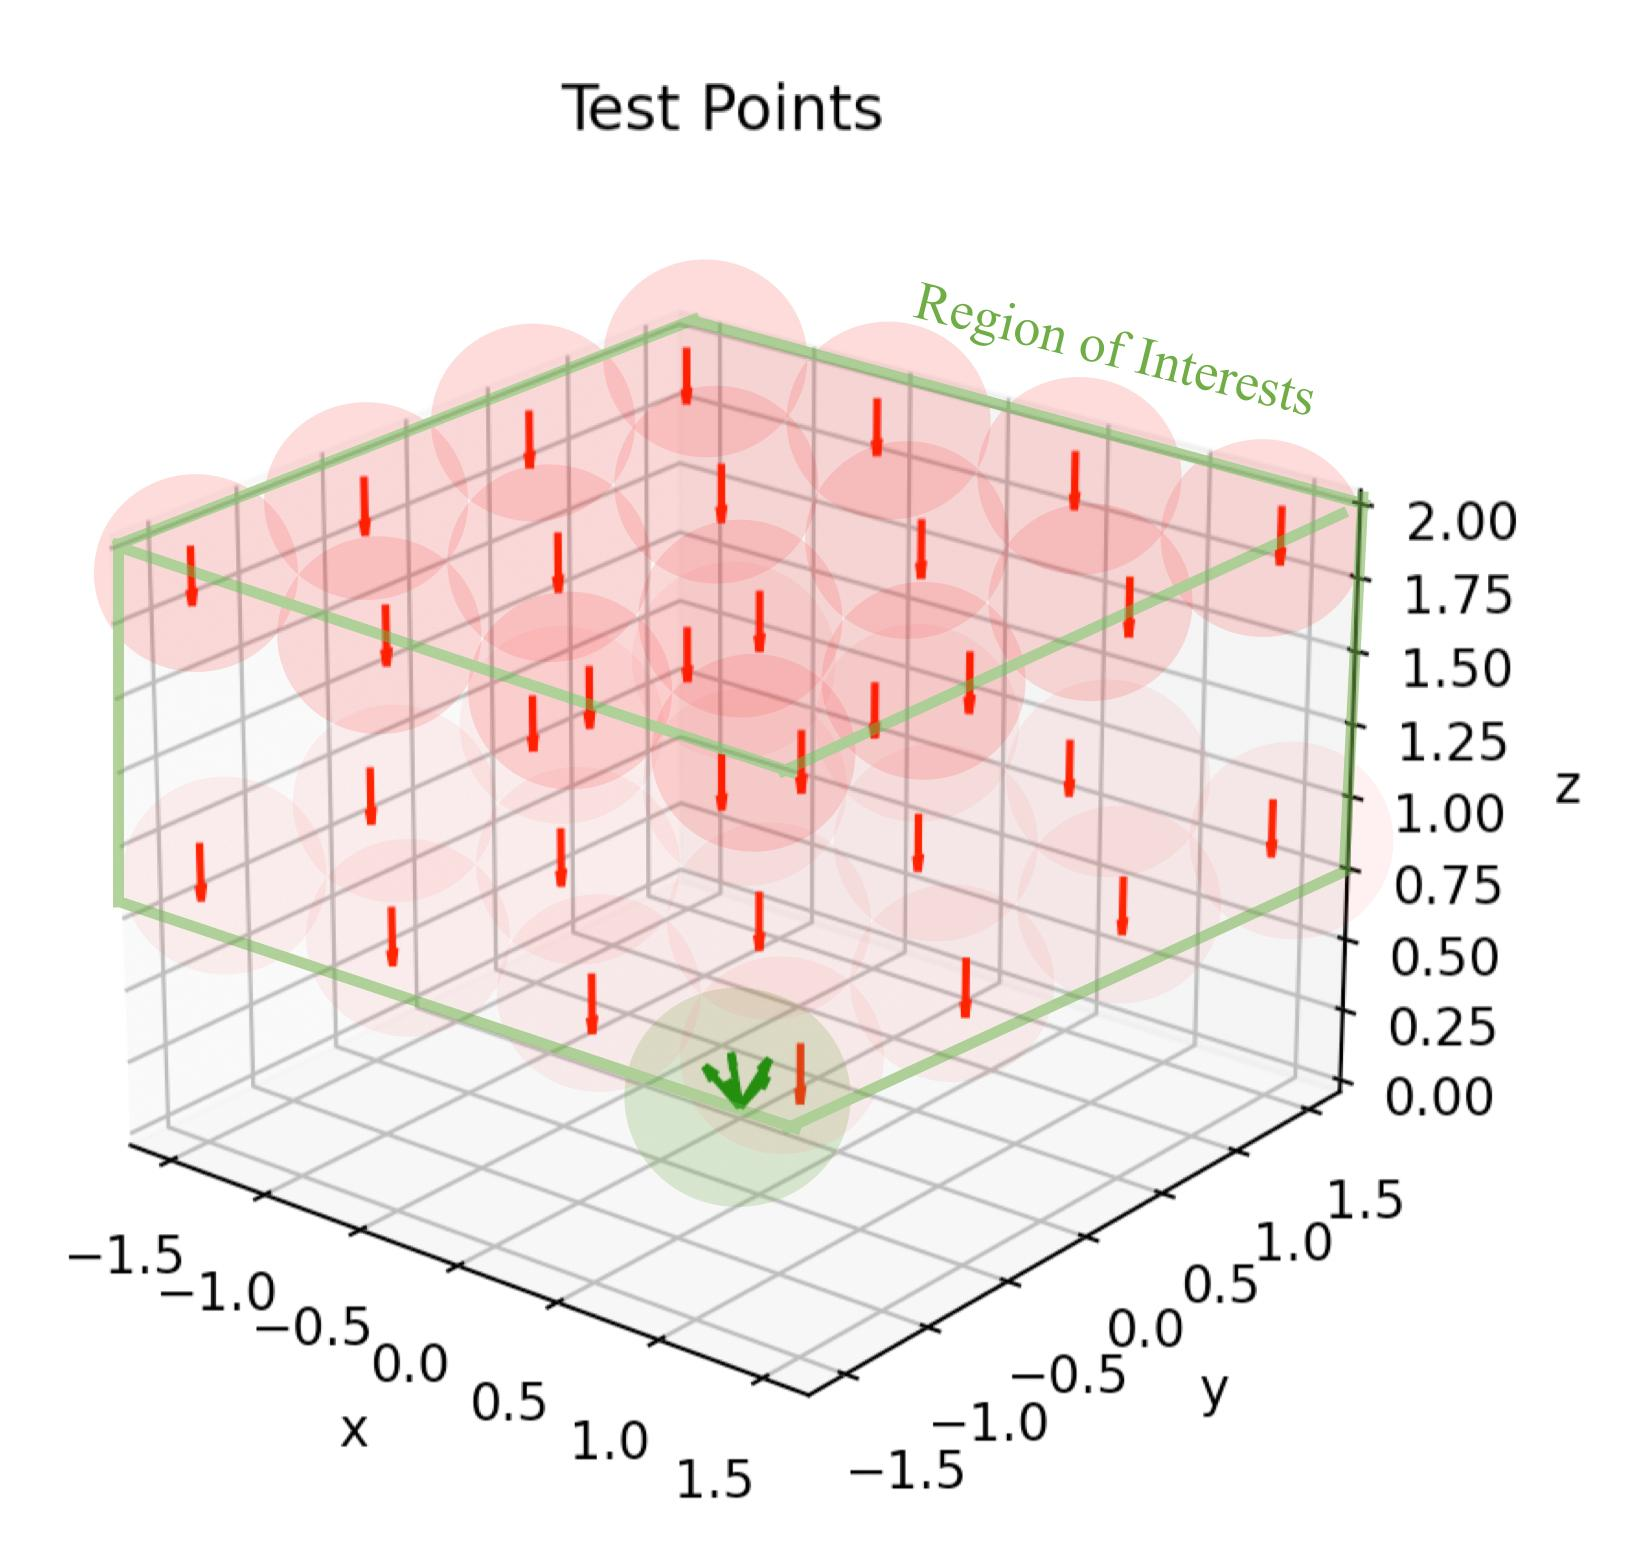
\includegraphics[width=8cm]{ch3pic/testpoint.jpg}
%     \caption{ROI與樣本點示意圖}
%     \label{pic:testpoint}
% \end{figure}

% \clearpage

% \subsection{目標函數}

% 愈改善之目標為系統表現,期望能降低系統在ROI中的平均量測誤差,因此由\ref{eqn:objective}表示,將$K$個樣本點中的模擬量測相對位置與標準相對位置相減後,總和除$K$則得平均誤差;其中標準相對位置,為各樣本點相對PD座標系的位置;而模擬量測位置則利用第三章的方式進行數據處理所得。



